\documentclass[12pt, a4paper]{article}
	\input{preambulo}
	%%\title{Lógica Matemática}
%\author{Apuntes del alumno: Javier López}
%\date{2020}
\begin{titlepage}
\centering
\vspace{1cm}
{\bfseries\LARGE Universidad Complutense de Madrid \par}
\vspace{1cm}
{\scshape\Large Facultad de Ciencias Matemáticas \par}
\vspace{2cm}
{\scshape\Huge Lógica Matemática \par}
\vspace{1cm}
{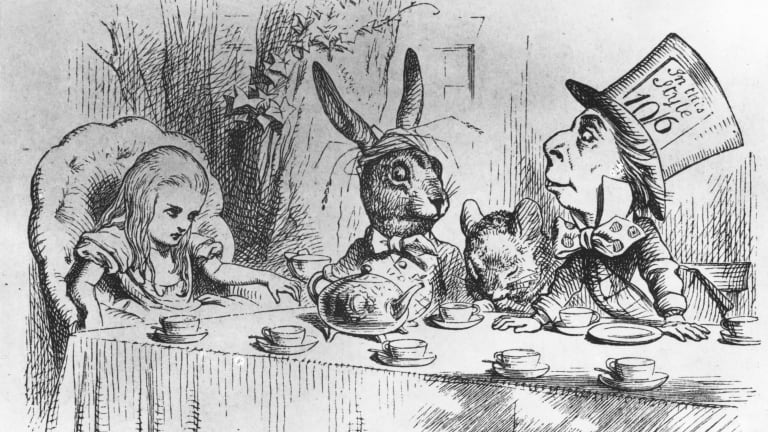
\includegraphics[width=0.7\textwidth]{alice.jpg}\par}
\vspace{3cm}
{\itshape\Large Curso académico 2019-2020 \par}
\vfill
{\Large Autor: Javier López \par}
\vfill
{\Large Versión Febrero 2020 \par}
\end{titlepage}  
        
\usepackage{vmargin}
	\setpapersize{A4}
\setmargins{2.5cm}       % margen izquierdo
{1.5cm}                        % margen superior
{16.5cm}                      % anchura del texto
{23.42cm}                    % altura del texto
{10pt}                           % altura de los encabezados
{1cm}                           % espacio entre el texto y los encabezados
{0pt}                             % altura del pie de página
{2cm}                           % espacio entre el texto y el pie de página        
        
\begin{document}

 %\title{Lógica Matemática}
%\author{Apuntes del alumno: Javier López}
%\date{2020}
\begin{titlepage}
\centering
\vspace{1cm}
{\bfseries\LARGE Universidad Complutense de Madrid \par}
\vspace{1cm}
{\scshape\Large Facultad de Ciencias Matemáticas \par}
\vspace{2cm}
{\scshape\Huge Lógica Matemática \par}
\vspace{1cm}
{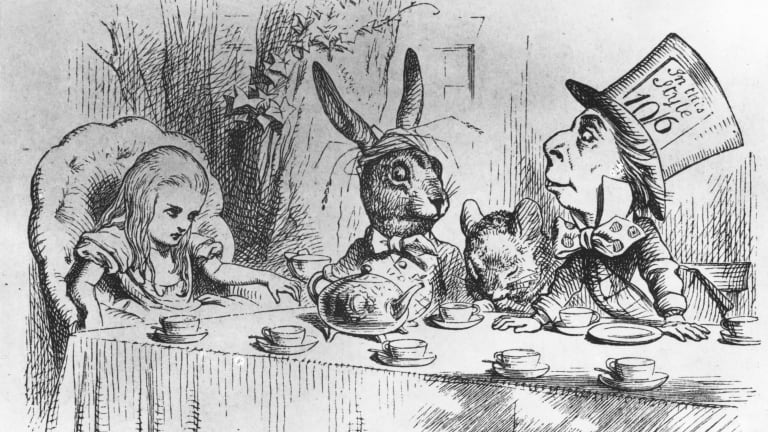
\includegraphics[width=0.7\textwidth]{alice.jpg}\par}
\vspace{3cm}
{\itshape\Large Curso académico 2019-2020 \par}
\vfill
{\Large Autor: Javier López \par}
\vfill
{\Large Versión Febrero 2020 \par}
\end{titlepage}
\newpage
\section*{Fe de errores}
\textit{Este texto está sacado íntegramente de los apuntes que he tomado en clase. Por ello, es más que probable, encontrar en él erratas y errores. Todos ellos pueden {\color{red} ser comunicados a través del foro del campus virtual de la asignatura} y serán subsanados lo antes posible o, en su defecto, añadidos a esta lista para que se tengan en cuenta}.
\begin{itemize}
	\item En el \textit{ejemplo III, el apartado $(\Box)$} no lo tengo escrito en mis apuntes y por tanto la solución no es de Luis. 
	\item Recomiendo revisar el \textit{ejemplo V, caso 4}. 
\end{itemize}
\newpage
\newcommand{\p}[0]{\mbox{PROP}_{SP}}
\newcommand{\cb}[0]{\{ \wedge, \, \lor \, \rightarrow, \, \leftrightarrow \}} 
\newcommand{\boox}[0]{\, \Box \,}

\theoremstyle{definition}
\newtheorem{definition}{Definición}
	%\tableofcontents
%	\maketitle
	\newpage
     \pagestyle{fancy}
        \setlength\headheight{23pt}
        \fancyhf{}
        \lhead{\bfseries Lógica matemática}
        \chead{}
        \rhead{UCM}
        \lfoot{Curso 19/20}
        \cfoot{}
        \rfoot{\thepage}
        \renewcommand{\headrulewidth}{0.1pt}
        \renewcommand{\footrulewidth}{0.1pt}
     %\newcommand{\p}[0]{\mbox{PROP}_{SP}}
%\newcommand{\cb}[0]{\{ \wedge, \, \lor \, \rightarrow, \, \leftrightarrow \}} 
%\newcommand{\boox}[0]{\, \Box \,}

\section*{Lógica de proposiciones}
\begin{definition} Diremos que una \textbf{proposición} es un enunciado que puede ser verdadero o falso. Nunca será una proposición cualquier enunciado que expresa duda o sentimientos. Tampoco lo serán aquellos enunciados que no tengan sentido lógico. 
\end{definition}
\paragraph{}
Un ejemplo de lo que no es proposición sería
\\
p $\equiv$ ``Juan se cae'' 
\\
q $\equiv$ ``Yo me río''
\\
$\varphi \equiv$ Juan se cae y yo me río  
\paragraph{}
\textbf{Conectivas lógicas}. Son los símbolos que utilizamos para formalizar las proposiciones. Estos son 
\[ \lnot \rightsquigarrow \mbox{ negación} \quad \wedge \rightsquigarrow \mbox{ conjunción} \quad 
\lor \rightsquigarrow \mbox{ disyunción} \quad \rightarrow \rightsquigarrow \mbox{ implicación} \quad
 \]  
 \[\leftrightarrow \rightsquigarrow \mbox{ implicación} \quad \bot \rightsquigarrow \mbox{ falso} \quad 
\top \rightsquigarrow \mbox{ cierto} \]

\begin{definition} Se denomina \textbf{formalizar} una proposición, a escribirla mediante conectivas lógicas. 
\end{definition}
\paragraph{}
\newcounter{ej} %creado el contador ejemplo
\addtocounter{ej}{1} % sumo 1
\textbf{Ejemplo \Roman{ej}}: Formalizar las siguientes frases 
\begin{enumerate}
	\item Si llueve se suspende el partido. 
	\item Solo si llueve se suspende el partido.
\end{enumerate}
tomando como proposiciones p $\equiv$ `` Llueve'' y q $\equiv$ ``se suspende el partido''.
\begin{itemize}
	\item[(1)] $ p\rightarrow q$
	\item[(2)] $ q\rightarrow p$
\end{itemize} 
\paragraph{}
\begin{definition} Llamaremos \textbf{formula} a una cadena de símbolos.
\end{definition}

\begin{definition} Denotamos el \textbf{conjunto de} todos los \textbf{símbolos de proposición} como 
	\[ \mbox{SP}=\{p, \, q, \ldots \} \]
	que es un conjunto numerable (no necesariamente finito). 
\end{definition}

\begin{definition} Al conjunto formado por SP y las conectivas lógicas se le denomina \textbf{alfabeto} y lo denotamos como 
	\[ \mbox{A}= \mbox{SP} \cup \{ \lnot, \, \wedge, \, \lor \, \rightarrow, \, \leftrightarrow, \, (, \, ) \} \]
	denotamos por $\mbox{A}^*$ al \textbf{conjunto de cadenas de símbolos} de A
	\[ \mbox{A}^*=\{ \varepsilon, \, a_1, \, a_2, \ldots , a_n : a_n \geq 0,\, a_i \in A,\, 1 \leq j \leq n   \} \]
	donde $\varepsilon$ es la cadena vacía. 
\end{definition}

\addtocounter{ej}{1} % sumo 1
\textbf{Ejemplo \Roman{ej}}: Dado el vocabulario $\mbox{A}=\{ a, \,b \}$ su conjunto de cadena de símbolos será el conjunto 
\[ \mbox{A}^*= \{\varepsilon, \, a, b, ab, ba, aaa, aab, \ldots \} \]
\begin{definition} Dado SP un conjunto de símbolos de proposición, tomamos el alfabeto $\mbox{A}_{SP}$ y definimos $\mbox{PROP}_{SP}$ como el menor subconjunto de $\mbox{A}^*_{SP}$ que verifica 
\begin{enumerate}
	\item $SP \subseteq \mbox{PROP}_{SP}$
	\item Si $\varphi \in \p$, entonces $(\lnot \varphi) \in \p$
	\item Si $\varphi, \psi \in \p$, entonces $(\varphi \, \Box \, \psi) \in \p$, donde \[ \Box \in \cb \] 
\end{enumerate}
\end{definition}
Veamos como se construye esta definición. Sean 
\[ P_0 = \mbox{SP} \]
\[ P_{n+1}= P_n \cup \{(\lnot \varphi), \, (\varphi \, \Box \, \psi) : \, \Box \in \cb, \, \varphi, \psi \in P_n \} \]
\[ P= \bigcup_{i \geq 0} \]
veamos como $P$ cumple las propiedades 1, 2 y 3 de la definición anterior. De forma trivial se verifica que $\p \subseteq P$ y nos faltaría por demostrar la inclusión en el otro sentido. 
\begin{proof}
Sea $\varphi \in P$ entonces $\exists k$ tal que $\varphi \in P_k$ y aplicamos inducción sobre $k$ para ver que $\varphi \in \p$. 
\paragraph{}
Para $k=0$, por la propiedad 1 de la definición se tienen que $\varphi \in \p$. Para $k \geq 0$ 
\begin{itemize}
	\item[(i)] $\varphi \in P_{k-1}$
	\item[(ii)] $\psi \in P_{k-1}$ tal que $\varphi = (\lnot \psi)$
	\item[(iii)] $\psi_1, \psi_2 \in P_{k-1}$ entonces $\varphi = (\psi_1 \boox \psi_2)$
\end{itemize}
\end{proof} %28/01/2020
     \subsection{Inducción estructural}
Supongamos que queremos probar una propiedad $P$ que cumpla $P(\varphi), \forall \varphi \in \p$. Para ello vamos a usar una estructura basada en el \textit{método de inducción} usual sobre $\mathbb{N}$ aplicado sobre las proposiciones. El método tiene la siguiente estructura 
\begin{itemize}
	\item[(1)] Demostrar la \textbf{base inductiva}. Lo haremos sobre las atómicas (\textit{i.e.} SP, $\bot, \top$)
	\begin{itemize}
		\item[(AT)] Se cumple $P(\varphi), \forall \varphi \in \mbox{AT}$.
	\end{itemize}
	\item[(2)] \textbf{Paso inductivo}. Una vez que tenemos la propiedad $P$ probada para el caso base, suponemos la cierta la hipótesis de inducción, es decir que se cumple $P(\varphi),$ y la utilizamos para los dos casos siguientes
	\begin{itemize}
		\item[$(\lnot \varphi)$] Utilizando la \textit{h.i.} demostraremos que se cumple $P((\lnot \varphi))$.
		\item[($\Box$)] Suponemos que $\varphi_1$ cumple $P$ y que $\varphi_2$ cumple $P$, es decir, se verifican $P(\varphi_1)$ y $P(\varphi_2)$ y entonces hay que demostrar $P(\varphi_1 \boox \varphi_2)$ con $\Box \in \cb$. Dependiendo de la propiedad que queramos demostrar, podremos, o bien agrupar la conectivas lógicas en un sólo caso, o bien separarlas de forma en casos particulares. 
	\end{itemize}
\end{itemize} 
\addtocounter{ej}{1} % sumo 1
\textbf{Ejemplo \arabic{ej}}: Vamos a demostrar por inducción estructural la siguiente propiedad
\begin{center}
P: \textit{Toda fórmula tiene el mismo número de paréntesis abiertos y cerrados}
\end{center}
Para ello, vamos a denotar $\vert \varphi \vert_{(}$ al número de paréntesis abiertos de $\varphi$ y, análogamente, denotamos $\vert \varphi \vert_{)}$ al número de paréntesis cerrados de $\varphi$.
\paragraph{}
\begin{itemize}
	\item[(AT)] Si $\varphi \in SP$ ó $\varphi=\bot$ ó $\varphi=\top$, en cualquiera de los casos no hay paréntesis, luego $\vert \varphi \vert_{(}=\vert \varphi \vert_{)}$ y por tanto se verifica
	\[ P(\varphi), \forall \varphi \in \mbox{AT} \]
	\item[$(\lnot \varphi)$] Sea $\varphi \in \p$ tal que se verifica $P(\varphi)$, es decir 
	\[ \vert \varphi \vert_{(}=\vert \varphi \vert_{)} \]
	ahora, el $\vert (\lnot \varphi) \vert_{(}= \vert \varphi \vert_{(} +1$ y analogamente $\vert (\lnot \varphi) \vert_{)}= \vert \varphi \vert_{)} +1$, luego por \textit{h.i.} se tiene que 
	\[ \vert (\lnot \varphi) \vert_{)}=\vert (\lnot \varphi) \vert_{(}  \]  
	luego se verifica $P(\lnot \varphi), \forall \varphi \in \p$.
	\item[($\Box$)] Sean $\varphi_1, \, \varphi_2 \in \p$, supongamos que
	\[ \mbox{Se verifica } P(\varphi_1) \Rightarrow \vert \varphi_1 \vert_{(}=\vert \varphi_1 \vert_{)}  \]
	\[ \mbox{Se verifica } P(\varphi_2) \Rightarrow \vert \varphi_2 \vert_{(}=\vert \varphi_2 \vert_{)}  \]  
	y veamos que ocurre con $P(\varphi_1 \boox \varphi_2)$ 
	\[ \vert \varphi_1 \boox \varphi_2 \vert_{(}= \vert \varphi_1 \vert_{(} + \vert \varphi_2 \vert_{(} +1  \]
	\[ \vert \varphi_1 \boox \varphi_2 \vert_{)}= \vert \varphi_1 \vert_{)} + \vert \varphi_2 \vert_{)} +1  \]
	y, por \textit{h.i.} se tiene que  
	\[ \vert \varphi_1 \boox \varphi_2 \vert_{)}= \vert \varphi_1 \boox \varphi_2 \vert_{(} \]
	finalizando así la demostración.
\end{itemize}

\begin{definition} Sea A un alfabeto y $\omega \in A^*$ decimos que $\omega'$ es \textbf{prefijo} de $\omega$ si $\exists \omega''$ tal que 
\[ \omega=\omega' \omega'' \]
con, $\omega=a_1 \ldots a_n$, entonces $\exists k, \, 0\leq k \leq n$ tal que $\omega'=a_1 \ldots a_k$. Diremos que $\omega'$ es \textbf{prefijo propio} si $\omega' \neq \varepsilon$ y $\omega' \neq \omega$. 
\end{definition}

\addtocounter{ej}{1} % sumo 1
\textbf{Ejemplo \arabic{ej}}: Sea $A=\{ a,\,b \}$ y $\omega=aababb$ entonces 
\begin{multicols}{2}
\begin{itemize}
	\item Si $k=0 \Rightarrow \omega'=\varepsilon$
	\item Si $k=1 \Rightarrow \omega'=a$
	\item Si $k=2 \Rightarrow \omega'=aa$
	\item Si $k=3 \Rightarrow \omega'=aab$
	\item Si $k=4 \Rightarrow \omega'=aaba$
	\item Si $k=5 \Rightarrow \omega'=aabab$
	\item Si $k=5 \Rightarrow \omega'=\omega$		
\end{itemize}
\end{multicols}
\addtocounter{ej}{1} % sumo 1
\textbf{Ejemplo \arabic{ej}}: Sea $\varphi'$ prefijo propio de $\varphi$, vamos a probar por inducción estructural la propiedad 
\begin{center}
P: \textit{El número de paréntesis cerrados de $\varphi'$ es menor que el número de paréntesis abiertos}.
\end{center}
utilizando la notación del ejemplo (III).
\begin{itemize}
	\item[(AT)] Sea $\varphi \in SP$, supongamos $\varphi=p$ entonces, o bien $\varphi'=\epsilon$ o $\varphi'=p$ luego $\varphi$ no tiene prefijos propios de modo que se cumple la propiedad. Si $\varphi=\bot$ o $\varphi = \top$ de nuevo $\varphi'=\epsilon$ o $\varphi'=\bot$ o $\varphi'=\top$ que no son prefijos propios, luego $\varphi$ tampoco tiene prefijos. 
	\[ P(\varphi), \forall \varphi \in \mbox{AT} \]
	\item[($\lnot \varphi$)] Supongamos que $\varphi'$ es prefijo propio de $(\lnot \varphi)$, y supongamos que todo prefijo propio de $\varphi$ cumple la propiedad. 
	\begin{itemize}
		\item[(CASO 1)] Si $\varphi'=($, entonces $\vert \varphi' \vert_{(}=1 > \vert \varphi' \vert_{)}=0$
		\item[(CASO 2)] Si $\varphi'=(\lnot$, entonces $\vert \varphi' \vert_{(}=1 > \vert \varphi' \vert_{)}=0$
		\item[(CASO 3)] Si $\varphi'=(\lnot \varphi''$, siendo $\varphi''$ prefijo de $\varphi$ luego cumple la propiedad, si además le sumamos uno la cumple también. 
		\item[(CASO 4)] Si $\varphi'=(\lnot \varphi$, entonces $\vert \varphi' \vert_{(}=1 = \vert \varphi' \vert_{)}=0 $
\end{itemize}	 
 \item[($\Box$)] Supongamos que todo prefijo propio de $\varphi_1$,  $\varphi_2$ cumple la propiedad. Hay que ver entonces, que los prefijos lo cumplen 
 \[(, \, (\varphi_1, \, \varphi_1, \, \varphi_1 \boox, \, (\varphi_1 \boox \varphi_2', \, (\varphi_1 \boox \varphi_2  \]
 \begin{flushright}
 \textit{Se deja como ejercicio}.
 \end{flushright}
\end{itemize} %29/01/2020
     \subsection*{Definiciones recursivas}
Supongamos que queremos definir una función 
\[ H: \p \rightarrow A \]
donde $A$ puede tomar diferentes tipos de conjunto: $\mathbb{N}$, $\mathcal{P}(\p)$,... para hacerlo de forma recursiva, vamos a necesitar las siguientes funciones auxiliares
\begin{itemize}
	\item Caso atómico
	\[ H_{\mbox{AT}}: \mbox{AT} \rightarrow A \]
dada por $H(\varphi)=H_{\mbox{AT}}(\varphi), \forall \varphi \in \mbox{AT}$
	\item Paso recursivo: donde diferenciamos entre la negación y las conectivas binarias. 
	\begin{itemize}
		\item[(i)] Negación 
		\[ H_{\lnot}: A \rightarrow A \]
		dada por 
	\[ H \vert (\lnot \varphi) \vert = H_{\lnot}\vert (H(\varphi) \vert \]
		\item[(ii)] Conectivas binarias 
		\[ H_{\Box}: A \times A \rightarrow A \]
		dada por 
	\[ H \vert (\varphi_1 \boox \varphi_2) \vert = H_{\Box}\vert (H(\varphi_1, \, \varphi_2) \vert \]
	\end{itemize}
\end{itemize} 
En los casos (i) e (ii) ni la entrada ni la salida de la función está formada por formulas. 
\paragraph{}
\addtocounter{ej}{1} % sumo 1
\textbf{Ejemplo \Roman{ej}}: Si queremos definir de forma recursiva el número de paréntesis abiertos de una proposición
\[ H_{(}: \p \rightarrow \mathbb{N} \] 
se tendría
\[ H_{\mbox{AT}\,(}: \mbox{AT} \rightarrow \mathbb{N} \]
dada por
\[ H_{\mbox{AT}\,(}(\varphi)=0, \forall \varphi \in \mbox{AT} \]
la negación
\[ \begin{matrix}
 H_{\lnot \,(}: & \mathbb{N} & \rightarrow & \mathbb{N}\\
 &n& \longmapsto &  n+1
\end{matrix} \] 
finalmente, el resto de conectivas 
\[ \begin{matrix}
 H_{\Box \,(} :  & \mathbb{N} \times \mathbb{N} & \rightarrow & \mathbb{N}\\
 &(n,\, m)& \longmapsto &  n+m+1
\end{matrix} \] 
Escribirlo así es un poco farragoso por lo que, generalmente, escribiremos las funciones haciendo uso del propio concepto de recursión
\[ H_{(}(\varphi)=0, \forall \varphi \in \mbox{AT} \]
\[ H_{\lnot \,(}((\neg \varphi))=H_{(}(\varphi) +1 \]
\[ H_{\Box \,(}(\varphi_1 \boox \varphi_2)= H_{(}(\varphi_1)+H_{(}(\varphi_2)+1 \]
además, en la escritura, se suprime la función auxiliar. 
\addtocounter{ej}{1} % sumo 1
\textbf{Ejemplo \Roman{ej}}: definiremos de forma recursiva el número de apariciones de $\wedge$ en $\varphi$ y lo denotamos como $\vert \varphi \vert^{\wedge}$.
\begin{itemize}
	\item[(AT)] $\vert \varphi \vert^{\wedge}=0, \forall \varphi \in \mbox{AT}$
	\item[($\neg$)] $\vert (\neg \varphi) \vert^{\wedge}=\vert \varphi \vert^{\wedge}$
	\item[($\Box$)] Hay que diferenciar dos casos
	\[ \vert (\varphi_1 \boox \varphi_2) \vert^{\wedge}= \left\lbrace \begin{matrix}
	\vert \varphi_1 \vert^{\wedge}+\vert \varphi_2 \vert^{\wedge}& \mbox{si}& \Box \in \{ \lor, \, \rightarrow, \, \leftrightarrow\}\\
	\\
	\varphi_1 \vert^{\wedge}+\vert \varphi_2 \vert^{\wedge}+1 & \mbox{si}& \Box=\wedge
\end{matrix} \right.	 \] 
\end{itemize}
\begin{definition} Dadas dos fórmulas $\varphi$ y $\psi$ decimos que $\psi$ es una \textbf{subformula} de $\varphi$ si una parte de $\varphi$ formada por símbolos consecutivos es idéntica a $\psi$.
\end{definition}
\addtocounter{ej}{1} % sumo 1
\textbf{Ejemplo \Roman{ej}}: dada la formula, 
\[ \varphi \equiv (p \lor (q \rightarrow (\neg r))) \]
observamos que esta formada por las subformulas siguientes
\[ p, \, q, \, r \, (\neg r), \, (q \rightarrow (\neg r)), \varphi \]
\addtocounter{ej}{1} % sumo 1
\textbf{Ejemplo \Roman{ej}}: Creamos una función recursiva que devuelva las diferentes subformulas de una formula dada.
\[ \mbox{SUB}: \p \rightarrow \mathcal{P}(\p) \]
dada por 
\begin{itemize}
	\item[(AT)] $\mbox{SUB}(\varphi)=\{\varphi \}, \forall \varphi \in \mbox{AT}$
	\item[($\neg$)] $\mbox{SUB}((\neg \varphi))=\{ (\neg\varphi)\} \cup \mbox{SUB}(\varphi)$
	\item[($\Box$)] $ \mbox{SUB} ((\varphi_1 \boox \varphi_2) )= \mbox{SUB}(\varphi_1)+\mbox{SUB}(\varphi_2) \cup \{ (\varphi_1 \boox \varphi_2) \}$
\end{itemize}
\begin{prop} El esquema de definición recursiva da como resultado una única función. Esto es, dadas 
\[ H_{\mbox{AT}}: \mbox{AT} \rightarrow A \]
\[ H_{\lnot}: A \rightarrow A \]
\[ H_{\Box}: A \times A \rightarrow A \]
existe una única función $H: \p \rightarrow A$ que verifica 
\[ H(\varphi)=H_{\mbox{AT}}(\varphi), \forall \varphi \in \mbox{AT} \]
\[H((\neg \varphi))=H_{\neg}(H (\varphi))\]
\[H ( (\varphi_1 \boox \varphi_2) ) = H_{\Box}(H(\varphi_1, \, \varphi_2))\]
\end{prop}
\subsection*{Eliminación de paréntesis}
Como en la aritmética básica, cuando escribimos una operación podemos utilizar las reglas de prioridad, asociatividad, etc. para escribir el menor número de paréntesis posible. Así por ejemplo en 
\[ (((2 \cdot 3)+5)-(3 \cdot 2))=2 \cdot 3 +5-3\cdot 3 \]
la idea es, por tanto, dar una serie de reglas para poder hacer lo mismo con nuestras formulas de proposición. 
\subsubsection*{Reglas de eliminación de paréntesis}
\begin{enumerate}
	\item \textbf{Elminación de paréntesis externos}. No aportan información.
	\item \textbf{Prioridad entre conectivas}. En la siguiente lista, las conectivas, aparecen de más prioridad a menos
	\[ (+)\quad \neg, \, \wedge, \, \lor, \, \rightarrow, \, \leftrightarrow \quad (-) \]
	\item \textbf{Asociatividad}. Adoptamos el convenio de asociar por la izquierda. De este modo si tenemos $p \rightarrow q \rightarrow r$ daremos como asociación válida 
	\[ (p \rightarrow q) \rightarrow r \]
	siendo, por tanto, errónea 
	\[ p \rightarrow (q \rightarrow r)  \]
	Esto mismo se aplica para $\leftrightarrow$. En los casos de $\vee$ y $\wedge$ no se presenta problema pues son asociativas.
\end{enumerate} %30/01/2020
%		\newpage     
	%     \input{clase5}
%		\newpage     
%     \includepdf[pages=-]{clase6}
%		\newpage     
%     \input{clase7}
%		\newpage     
%     \input{clase8}
%     	\newpage
%     \input{clase9}
%     	\newpage
%     \input{clase10}
%     	\newpage
%     \input{clase11} 
%     	\newpage
%     \input{clase12} 
%     	\newpage
%     \input{clase13} 
\end{document}